\section{Empirical Risk Minimization}

\mode<presentation>{
\begin{frame} 
    \begin{center} \huge
        \secname
    \end{center}
    \begin{center}
    Optimize the cost function using training data.
    \end{center}
\end{frame}
}

\begin{frame}{Our model for solving the ICA problem}

Consider the following perceptron network with $N$ inputs and $N$ outputs:
\begin{figure}[ht]
\centering
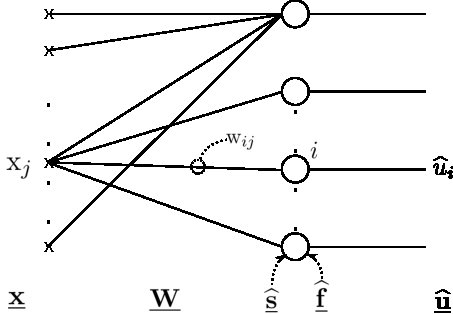
\includegraphics[width=4.5cm]{img/section2_fig16}
%\caption{$N-N$ perceptron network}
\end{figure}
where
\svspace{-4mm}
\begin{equation}
\widehat{u}_i := \widehat{f}_i 
	\big( 
		s_i 
	\big) = \underbrace{
	\widehat{f}_i 
	\Big( \sum_{j=1}^{N} \mathrm{w}_{ij} 
		\mathrm{x}_j 
	\Big) }_{
	\substack{
		\text{often a} \\
		\text{sigmoid function}\\
		\text{or\;} \tanh}
	}
\end{equation}
and observations:
\svspace{-4mm}
\begin{equation}
\vec{x}^{(\alpha)} \in \mathbb{R}^N, 
		\quad \alpha = 1, \ldots, p
\end{equation}
The weights $w_{ij}$ will be determined through inductive learning.

\end{frame}

\begin{frame}

Deriving the cost function for this network to find the Infomax solution:
\begin{equation}
\label{eq:conservationvec}
	P_{\vec{u}} (\widehat{\vec{u}}) d \widehat{\vec{u}}
		= P_{\vec{x}}(\vec{x}) d \vec{x}
\end{equation}
\begin{align}
\label{eq:uxj}
	P_{\vec{u}} (\widehat{\vec{u}}) 
	& = \left| \det \frac{d \vec{x}}{d \widehat{\vec{u}}} \right|
		P_{\vec{x}}(\vec{x}) \\
	& = \frac{P_{\vec{x}}(\vec{x})}{ \left| \det
		\frac{d \widehat{\vec{u}}}{d \vec{x}} \right|}\\
    & = \frac{P_{\vec{x}}(\vec{x})}{|\det \vec{J}\,|}
\end{align}
with elements of the Jacobian $\vec J$ given as
\slidesonly{
	\begingroup
	\small
}
\begin{align}
\label{eq:jacobelement}
 J_{ij}=
 \frac{\partial \widehat{u}_i}{\partial \mathrm{x}_j}
	& = \frac{\partial}{\partial \mathrm{x}_j} 
		\widehat{f}_i \bigg( \sum\limits_{k = 1}^N \mathrm{w}_{ik} 
		\mathrm{x}_k \bigg) \notesonly{\\
	&} = \mathrm{w}_{ij} \widehat{f}_i^{'} \bigg( \sum\limits_{k = 1}^N 
		\mathrm{w}_{ik} \mathrm{x}_k \bigg).
\end{align}
\slidesonly{
	\endgroup
}

We therefore obtain for the value of the Jacobian determinant
\slidesonly{
	\begingroup
	\footnotesize
}
\begin{equation} \label{eq:functionalDeterminant}
|\det \vec {J}\,| = 
	\Big| \det \frac{\partial \widehat{\vec{u}}}{\partial \vec{x}} \Big|
	= |\det \vec{W}\, | \prod\limits_{l = 1}^N  \widehat{f}_l^{'} \Bigg( 
		\sum\limits_{k = 1}^N \mathrm{w}_{lk} \mathrm{x}_k \Bigg).
\end{equation}
\slidesonly{
	\endgroup
}

\end{frame}

\clearpage

\begin{frame}

\slidesonly{
\visible<1->{
\vspace{-7mm}
\hspace{8.0cm}
\StickyNote[1.7cm]{
	\begingroup
	\scriptsize
\begin{equation}
%\label{eq:conservationvec}
	P_{\vec{u}} (\widehat{\vec{u}}) d \widehat{\vec{u}}
		= P_{\vec{x}}(\vec{x}) d \vec{x}
\end{equation}
\begin{equation}
%\label{eq:uxj}
	P_{\vec{u}} (\widehat{\vec{u}}) 
	= \frac{P_{\vec{x}}(\vec{x})}{|\det \vec{J}\,|}
\end{equation}
	\endgroup
}[3.cm] % width
\vspace{-22mm}
}
}

\notesonly{Inserting \eqref{eq:conservationvec} and \eqref{eq:uxj} into the Infomax cost function from \eqref{eq:infomax} gives} 
\begin{eqnarray}
H & = & -\int d \widehat{\vec{u}} P_{\vec{u}} (\widehat{\vec{u}})
  \ln P_{\vec{u}} (\widehat{\vec{u}}) \\
& = &  
-\int d \vec{x} P_{\vec{x}} (\vec{x}) \ln \frac{P_{\vec{x}}(\vec{x})}{|\det \vec{J}\,|} \\
& = & 
\underbrace{
    -\int d \vec{x} P_{\vec{x}} (\vec{x}) \ln P_{\vec{x}}(\vec{x})
}_{ \text{constant w.r.t. } \vec W } 
    + \int d \vec{x} P_{\vec{x}} (\vec{x}) \ln |\det \vec{J}\,|
\end{eqnarray}
and with \notesonly{\eqref{eq:functionalDeterminant}}
\slidesonly{
	\begingroup
	\footnotesize
}
\begin{equation} \label{eq:functionalDeterminant}
|\det \vec {J}\,| = 
	\Big| \det \frac{\partial \widehat{\vec{u}}}{\partial \vec{x}} \Big|
	= |\det \vec{W}\, | \prod\limits_{l = 1}^N  \widehat{f}_l^{'} \Bigg( 
		\sum\limits_{k = 1}^N \mathrm{w}_{lk} \mathrm{x}_k \Bigg).
\end{equation}
\slidesonly{
	\endgroup
}
we can formulate the cost 
in terms that depend on components in $\vec W$:
\begin{equation}
	H =~\text{const.} \, + \; \ln |\det \vec{W}\,| \underbrace{\int d \vec{x} P_{\vec{x}} (\vec{x})}_{=\,1}
		+ \int d \vec{x} P_{\vec{x}} (\vec{x}) \sum\limits_{l = 1}^N
			\ln \widehat{f}_l^{'} \Bigg( \sum\limits_{k = 1}^N 
			\mathrm{w}_{lk} \mathrm{x}_k \Bigg).
\end{equation}

\end{frame}

\begin{frame}{Generalization cost}

\only<1>{
\slidesonly{
\begin{equation}
	H =~\text{const.} \, + \; \ln |\det \vec{W}\,| \underbrace{\int d \vec{x} P_{\vec{x}} (\vec{x})}_{=\,1}
		+ \int d \vec{x} P_{\vec{x}} (\vec{x}) \sum\limits_{l = 1}^N
			\ln \widehat{f}_l^{'} \Bigg( \sum\limits_{k = 1}^N 
			\mathrm{w}_{lk} \mathrm{x}_k \Bigg).
\end{equation}
}
}


This enables us to define the generalization cost $E^G$ for model selection:
\begin{equation} \tag{generalization cost}
	E^G = \ln |\det \vec W\,| + \int d \vec{x} P_{\vec{x}} (\vec{x})
		\Bigg\{ \sum\limits_{l = 1}^N \ln
			\widehat{f}_l^{'} \Bigg( \sum\limits_{k = 1}^N 
			\mathrm{w}_{lk} \mathrm{x}_k \Bigg)
		\Bigg\}
\end{equation}

\only<2>{
The \emph{principle of empirical risk minimization} (in our particular case maximization) allows
\begin{center}
mathematical expectation $E^G \longrightarrow$ empirical average $E^T$
\end{center}
the \emph{training cost}
\begin{equation} \label{eq:trainingCost}
	E^T = \ln |\det \vec{W}\,| + \frac{1}{p} \sum\limits_{\alpha = 1}^p
		\sum\limits_{l = 1}^N \ln \widehat{f}_l^{'} \Bigg( 
		\sum\limits_{k = 1}^N \mathrm{w}_{lk} 
		\mathrm{x}_k^{(\alpha)} \Bigg)
\end{equation}
can be used for model selection using empirical data 
\begin{equation}
E^T \eqexcl \max_{\vec W}
\end{equation}
}

\end{frame}

\newpage
